\documentclass{minimal}

\usepackage{tikz}
\usetikzlibrary{calc, arrows, fit, positioning}
\definecolor{clamped}{RGB}{200,200,200}

\begin{document}
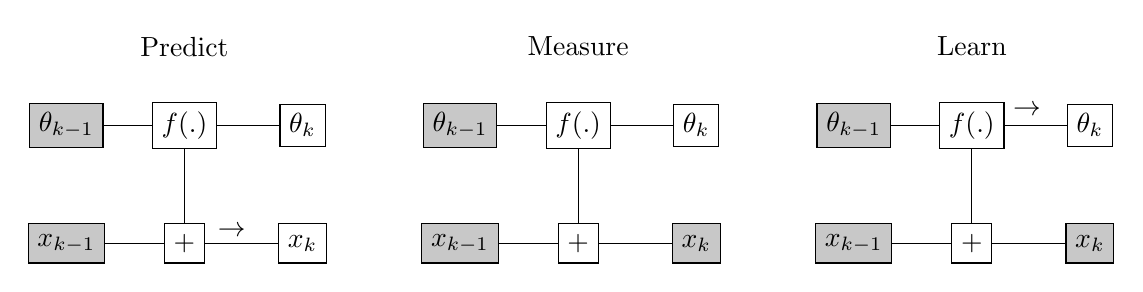
\begin{tikzpicture}
    [
        node distance=15mm,auto,>=latex',
        box/.style={draw, minimum size=.5cm},
        bbox/.style={draw, minimum size=1cm},
        blackbox/.style={draw, fill=black, minimum size=0.25cm}
    ]
    \tikzstyle{line} = [draw, -latex,>=latex]
    \tikzstyle{dash} = [dashed, -latex,>=latex]
    \tikzstyle{branch} = [fill,shape=circle,minimum size=3pt,inner sep=0pt]
    
    % Predict
    \begin{scope}
        \node[box] (f) {$f(.)$};
        \node[box, left of=f, fill=clamped] (theta_k_min) {$\theta_{k-1}$};
        \node[box, right of=f] (theta_k) {$\theta_{k}$};
        \node[box, below of=f, label={[shift={(0.6cm,-0.3cm)}]$\rightarrow$}] (add) {+};
        \node[box, left of=add, fill=clamped] (x_k_min) {$x_{k-1}$};
        \node[box, right of=add] (x_k) {$x_{k}$};

        \path[line] (f) edge[-] (add);
        \path[line] (f) edge[-] (theta_k_min);
        \path[line] (f) edge[-] (theta_k);
        \path[line] (add) edge[-] (x_k_min);
        \path[line] (add) edge[-] (x_k);

        \node[above of=f, node distance=1.0cm] {Predict};
   \end{scope}

    % Measure
    \begin{scope}[shift={(5.0cm, 0.0cm)}]
        \node[box] (f) {$f(.)$};
        \node[box, left of=f, fill=clamped] (theta_k_min) {$\theta_{k-1}$};
        \node[box, right of=f] (theta_k) {$\theta_{k}$};
        \node[box, below of=f] (add) {+};
        \node[box, left of=add, fill=clamped] (x_k_min) {$x_{k-1}$};
        \node[box, right of=add, fill=clamped] (x_k) {$x_{k}$};

        \path[line] (f) edge[-] (add);
        \path[line] (f) edge[-] (theta_k_min);
        \path[line] (f) edge[-] (theta_k);
        \path[line] (add) edge[-] (x_k_min);
        \path[line] (add) edge[-] (x_k);

        \node[above of=f, node distance=1.0cm] {Measure};
   \end{scope}

    % Learn
    \begin{scope}[shift={(10.0cm, 0.0cm)}]
        \node[box, label={[shift={(0.7cm,-0.3cm)}]$\rightarrow$}] (f) {$f(.)$};
        \node[box, left of=f, fill=clamped] (theta_k_min) {$\theta_{k-1}$};
        \node[box, right of=f] (theta_k) {$\theta_{k}$};
        \node[box, below of=f] (add) {+};
        \node[box, left of=add, fill=clamped] (x_k_min) {$x_{k-1}$};
        \node[box, right of=add, fill=clamped] (x_k) {$x_{k}$};

        \path[line] (f) edge[-] (add);
        \path[line] (f) edge[-] (theta_k_min);
        \path[line] (f) edge[-] (theta_k);
        \path[line] (add) edge[-] (x_k_min);
        \path[line] (add) edge[-] (x_k);

        \node[above of=f, node distance=1.0cm] {Learn};
   \end{scope}

\end{tikzpicture}
\end{document}